\let\negmedspace\undefined
\let\negthickspace\undefined
\documentclass[journal]{IEEEtran}
\usepackage[a5paper, margin=10mm, onecolumn]{geometry}
\usepackage{lmodern} % Ensure lmodern is loaded for pdflatex
 % Include tfrupee package
\setlength{\headheight}{1cm} % Set the height of the header box
\setlength{\headsep}{0mm}     % Set the distance between the header box and the top of the text
\usepackage{enumitem}
\usepackage{gvv-book}
\usepackage{gvv}
\usepackage{cite}
\usepackage{amsmath,amssymb,amsfonts,amsthm}
\usepackage{algorithmic}
\usepackage{graphicx}
\usepackage{textcomp}
\usepackage{xcolor}
\usepackage{txfonts}
\usepackage{listings}
\usepackage{enumitem}
\usepackage{mathtools}
\usepackage{gensymb}
\usepackage{comment}
\usepackage[breaklinks=true]{hyperref}
\usepackage{tkz-euclide} 
\usepackage{listings}
% \usepackage{gvv}                                        
\def\inputGnumericTable{}                                 
\usepackage[latin1]{inputenc}                                
\usepackage{color}                                            
\usepackage{array}                                            
\usepackage{longtable}                                       
\usepackage{calc}                                             
\usepackage{multirow}                                         
\usepackage{hhline}                                           
\usepackage{ifthen}                                           
\usepackage{lscape}
\begin{document}

\bibliographystyle{IEEEtran}
\vspace{3cm}

\title{3-3-9}
\author{AI24BTECH11008- Sarvajith
}
% \maketitle
% \newpage
% \bigskip
{\let\newpage\relax\maketitle}

\renewcommand{\thefigure}{\theenumi}
\renewcommand{\thetable}{\theenumi}
\setlength{\intextsep}{10pt} % Space between text and floats
\numberwithin{equation}{enumi}
\numberwithin{figure}{enumi}
\renewcommand{\thetable}{\theenumi}
\textbf{Question: }\\
Draw an isosceles triangle ABC in which BC = 5.5cm and altitude AL = 5.3cm. \\
\textbf{Solution: }\\
\renewcommand{\tablename}{TABLE 1}
\begin{table}[h!]    
\centering
 \begin{tabular}{|c|c|}
\hline
\textbf{lengths} & \textbf{values}\\
\hline
\textbf{BC} & 5.5cm\\
\hline
\textbf{AL} & 5.3cm\\
\hline
\end{tabular}

\caption{values of lengths of triangle}
 \label{tab1-1.2-18-1}
\end{table}
The vertices of the above triangle are given by:
\begin{align}
    \textbf{A} &= c\myvec{\cos B\\\sin B} \label{eq. 3-3-9.1}\\
    \textbf{B} &= \myvec{0\\0}\label{eq. 3-3-9.2}\\
    \textbf{C} &= \myvec{a\\0}\label{eq. 3-3-9.3}
\end{align}
Where a,b,c are BC,AB,AC respectively and B is the angle formed by the side AB and BC.\\
AL bisects BC, then 2 right angled triangle ALB and ALC are formed.\\
from the pythogoras theorem 
\begin{align*}
    AB^2 &= AL^2 + BL^2\\
    c^2  &= 5.3^2 + 2.75^2\\
    c    &= \sqrt{35.65} \\c &= 5.97\\
    \cos B &= \frac{BL}{c}&= 0.46\\
    \sin B &= \frac{AL}{c}&= 0.88\\
\end{align*}
 substituting the above values \ref{eq. 3-3-9.1},\ref{eq. 3-3-9.3}\\
\begin{align*}
     \textbf{A}&=\myvec{2.75\\5.3}\\
     \textbf{B}&=\myvec{0\\0}\\
     \textbf{C}&=\myvec{5.5\\0}
\end{align*}




\begin{figure}[h!]
\centering
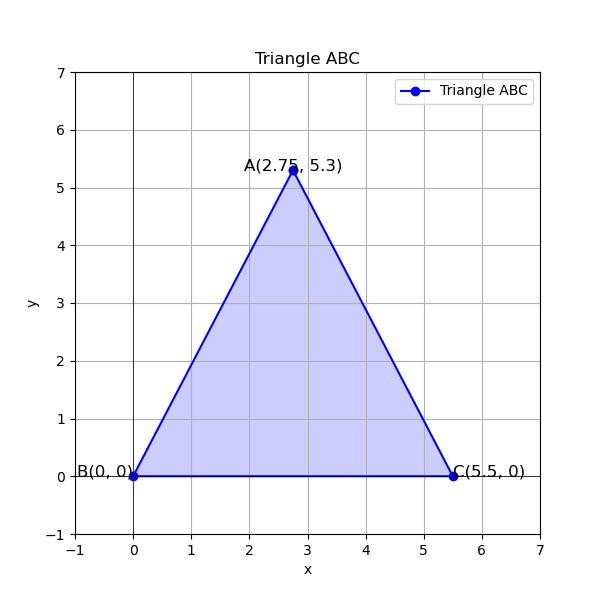
\includegraphics[width=0.7\columnwidth]{figs/Figure_1.png}
\caption{plot for isosceles triangle}
 \label{fig. 3-3-9-1}
\end{figure}
\end{document}

